\section{Ejecución simbólica dinámica}

\section{Blockchains}
Una blockchain es una base de datos pública, distribuida e inmutable.
Las transacciones se agrupan en conjuntos de \textit{bloques}, que son la unidad mínima con la que se actualiza el estado de la blockchain.
El historial de bloques agregados a la blockchain (y por ende, las transacciones ejecutadas) es público, y el estado actual de la red puede calcularse a partir de este historial.

Las redes de blockchain, al ser sistemas distribuidos, cuentan con protocolos de consenso para que las partes participantes puedan acordar cuál es el estado actual de la red.
La elección de protocolo de consenso es uno de los elementos más decisivos con respecto a una blockchain, y suelen estar pensados para garantizar propiedades de seguridad criptográfica sobre su estado \cite{bitcoin-backbone-protocol}\cite{ouroboros-protocol}\cite{survey-on-protocols}.
Ethereum, que será la tecnología de blockchain de la que hablaremos de aquí en adelante, cambió el protocolo de su red principal desde un protocolo Proof-of-Work llamado \texttt{Ethash} hacia un protocolo Proof-of-Stake denominado \texttt{Gasper} el 15 de Septiembre de 2022 en un proceso apodado ``The Merge'' (``La Fusión'') \cite{survey-of-blockchain-security} \cite{ethereum-yellow-paper} \cite{gasper-protocol} \cite{the-ethereum-merge}.
Desde la funcionalidad de los contratos inteligentes este evento es mayoritariamente un detalle; lo único que es pertinente saber es que a fines prácticos se considera que en Ethereum es imposible que ningún actor controle el ingreso de, o altere, la información en la red.

\subsection{Contratos Inteligentes en Ethereum y Solidity}
A continuación explicaremos los aspectos relevantes de la arquitectura de la red Ethereum.
Queremos abordar cómo los contratos inteligentes existen en ella, y cuáles son las peculiaridades de su ejecución.
Más adelante, explicaremos las características del lenguaje Solidity y las abordaremos con un ejemplo.

Las transacciones en Ethereum se refieren a propiedades sobre \textit{direcciones}, como el balance de criptomonedas o el estado de los contratos inteligentes.
Los contratos inteligentes se corresponden con direcciones dentro de la blockchain, de la misma forma que se corresponden con direcciones los usuarios ``humanos''.
De hecho, en Ethereum los contratos inteligentes y los usuarios tradicionales cuentan con dos tipos de \textit{accounts} distintas, que pueden pertenecer a usuarios humanos por un lado o a contratos inteligentes por el otro.
En el caso de los usuarios humanos el almacenamiento que le corresponde a cada dirección guarda sólo información sobre el balance de criptomonedas, mientras que un contrato inteligente utiliza dos campos adicionales: el \texttt{codeHash}, que es utilizado para obener el código ejectuable del contrato y el \texttt{storageRoot}, que es necesario para conocer una especie de memoria persistente exclusiva del contrato.
Ambos tipos de account pueden recibir o enviar mensajes y Ether\footnote{Ether es la criptomoneda utilizada por Ethereum.}.
La diferencia en los dos tipos radica en qué ocurre cuando la account es seleccionada como destinataria de una transacción.
Para las accountes de usuarios humanos simplemente se registra el suceso en la blockchain.
En el caso de un contrato inteligente, el momento de recibir una transacción es el momento en el que el programa se ejecuta, y el mensaje que dispara la ejecución es utilizado como los parámetros de entrada de la misma.
Para poder incluir la transacción en el próximo estado de la blockchain, el minero\footnote{Los ``mineros'' son quienes participan en el protocolo de la blockchain y registran las transacciones en bloques.} que registre la transacción debe levantar la EVM y simular la ejecución del contrato para conocer su estado final.

La EVM es una máquina de pila casi turing completa.
El lenguaje assembly asociado cuenta con instrucciones para números enteros, instrucciones para control de flujo y otras instrucciones referentes a particularidades de la ejecución en blockchain, como el contenido de las transacciones de la misma \cite{evm-opcodes}.
A pesar de que el conjunto de programas expresablas en el lenguaje de la EVM es turing completo, la cantidad de operaciones que se pueden ejecutar dentro de una única transacción están limitadas artificialmente por la cantidad de \textit{gas} asociado a la transacción.

El gas es una unidad de medida del esfuerzo de cómputo, y está ideado como elemento limitante de lo que se les permite hacer a los contratos inteligentes en Ethereum.
Debido a que los mineros deben ejecutar los contratos inteligentes en hardware y con recursos de los que ellos son dueños, el gas asociado a una transacción permite conocer cuánto deben pagarles los remitentes a los mineros por incluir las transacciones en un bloque.
Para controlar este costo, los remitentes de transacciones pueden establecer una cota superior al gas que tienen pensado gastar, al mismo tiempo que pueden ofertar distintos montos de criptomonedas por unidad de gas gastada.
Por otro lado, existe una cota superior a la cantidad de gas que tiene permitido consumir una transacción, lo que significa que una ejecución dada de la EVM siempre termina en un número finito de instrucciones.

En la actualidad, existen lenguajes utilizados para programar contratos en la red Ethereum.
De ellos, el que más adopción que tiene actualmente es Solidity.
Es un lenguaje imperativo curly-brace que provee una sintaxis similar a la de las clases en lenguajes orientados a objetos.
La sintaxis de Solidity incluye variables de estado, un método constructor, métodos internos (ejecutables sólo por el mismo contrato), y  un conjunto de métodos externos que representan la interfaz con otros contratos y el mundo, con la que los usuarios pueden interactuar.

\subsection{Ejemplo}
En el fragmento de código \ref{fig:solidity-example} presentamos un ejemplo de un programa escrito en Solidity, \texttt{SimpleMarketplace}\footnote{Este contrato es extraido de los contratos de ejemplo ``Mircrosoft Azure Blockchain Workbench'' \cite{azure-benchmark}}, el cual implementa un mecanismo simple para vender un bien.
A continuación haremos un breve análisis línea por línea del contrato.

En la línea 2 podemos ver que se define un tipo \textcolor{cyan}{\texttt{enum}} ``\texttt{StateType}'' que tiene tres valores posibles; que representan estados de completitud de la venta.
Las líneas 3 a 8 definen las variables de estado del contrato, entre las que tenemos variables de tipo \texttt{int}, \texttt{StateType} y \texttt{address}, indicando además mediante la palabra clave \textcolor{blue}{\texttt{public}} que estas variables resultan accesibles a contratos externos.
El tipo \texttt{address} utilizado en las variables \texttt{InstanceOwner} y \texttt{InstanceBuyer} consiste en valores enteros de 20 bytes de tamaño, y se utiliza para representar direcciones en la blockchain.

\begin{lstlisting}[language=Solidity, label={fig:solidity-example}, caption={Contrato Inteligente \texttt{SimpleMarketplace} en Solidity},captionpos=b]
pragma solidity >=0.4.25 <0.9.0;
pragma experimental ABIEncoderV2;

contract SimpleMarketplace {

    enum StateType {ItemAvailable, OfferPlaced, Accepted}
    address public InstanceOwner;
    string public Description;
    int public AskingPrice;
    StateType public StateEnum;  
    address public InstanceBuyer;
    int public OfferPrice;

    constructor(string memory description, int price, address sender) public
    {
        InstanceOwner = sender;
        AskingPrice = price;
        Description = description;
        StateEnum = StateType.ItemAvailable;
    }

    function MakeOffer(int offerPrice) public
    {
        require (offerPrice != 0 && StateEnum == StateType.ItemAvailable && InstanceOwner != msg.sender);
        InstanceBuyer = msg.sender;
        OfferPrice = offerPrice;
        StateEnum = StateType.OfferPlaced;
    }

    function Reject() public
    {
        require (StateEnum == StateType.OfferPlaced && InstanceOwner == msg.sender);
        StateEnum = StateType.ItemAvailable;
    }

    function AcceptOffer() public
    {
        require (StateEnum == StateType.OfferPlaced && msg.sender == InstanceOwner);
        StateEnum = StateType.Accepted;
    }
}
\end{lstlisting}

Observando el método \textcolor{blue}{\texttt{constructor}} de \texttt{SimpleMarketplace}, que es el método que siempre se llama al desplegar una instancia del contrato, vemos que define el objeto que se planea vender, indicando la descripción, el precio del producto y la dirección de su dueño actual \footnote{En la definición de \textcolor{blue}{\texttt{constructor}}, la palabra clave \textcolor{blue}{\texttt{memory}} indica qué estrategia debe usarse para sostener en memoria el string que entra por parámetro. Otras opciones, como \textcolor{blue}{\texttt{calldata}}, impactan en el costo de gas de la función.}.
Luego, las líneas 20, 28 y 34 indican precondiciones de los métodos \textcolor{orange}{\texttt{MakeOffer}}, \textcolor{orange}{\texttt{Reject}} y \textcolor{orange}{\texttt{AcceptOffer}}.
En ellas, la expresión \textcolor{magenta}{\texttt{msg.sender}} se refiere a la dirección desde la que se envió el mensaje que disparó la ejecución actual del contrato.
Si prestamos atención y debido a que el valor inicial de \texttt{SateEnum} es \texttt{ItemAvailable}, el único método que está permitido llamar inmediatamente después del constructor es \textcolor{orange}{\texttt{MakeOffer}}.
Mediante este, un potencial comprador puede realizar ofertas sobre el producto indicando un precio, que luego el dueño puede aceptar o rechazar.
Si el dueño original no está satisfecho con la oferta puede rechazarla llamando a \textcolor{orange}{\texttt{RejectOffer}}, regresando al estado incial en el que se aceptan nuevas ofertas.
Si eventualmente al dueño le interesa la última oferta realizada y la acepta, llama a \textcolor{orange}{\texttt{AcceptOffer}} y termina satisfactoriamente la ejecución del contrato, ya que
a partir de ese estado ningún otro método se encuentra habilitado. Los detalles de la venta realizada permanecen expuestos en las variables públicas del contrato, que a pesar de quedarse bloqueado a nuevos llamados a métodos permanece visible en la blockchain.


\section{Enabledness-Preserving Abstractions}


Una EPA es un Labeled Transition System (LTS) finito que busca abstraer el comportamiento de un contrato inteligente agrupando los estados del contrato en base a cuáles de sus metodos están habilitados \cite{de-caso-epa}.
Las transiciones en estos LTS representan el llamado a una función del contrato, indicando cómo un llamado a una función puede transformar el contrato de un estado abstracto a otro.

Comenzando por un ejemplo, en la figura \ref{fig:epa-example} presentamos la EPA del contrato \texttt{Simple\-Marketplace}.
El estado inicial, denominado \textbf{A}, está etiquetado \texttt{init} e indica el estado ``vacío'' previo al llamado al constructor del contrato.
Lo que podemos ver es que luego de ejecutar el método constructor se transiciona en la EPA a un único otro estado, al que llamamos \textbf{B}.
Allí, la etiqueta \texttt{\_MakeOffer} indica que \textcolor{orange}{\texttt{MakeOffer}} es el único método que se encuentra habilitado en \textbf{B}.
La única transición desde \textbf{B}, etiquetada \textcolor{orange}{\texttt{MakeOffer}}, indica lo que ocurre cuando se ejecuta ese método desde ese estado. Como vemos, seguir esa transición nos traslada  al estado \textbf{C}, que es un estado del contrato en el que solamente \textcolor{orange}{\texttt{AcceptOffer}} y \textcolor{orange}{\texttt{Reject}} se encuentran habilitados.
Luego, desde el estado \textbf{C} podemos ejecutar cualquiera de los dos métodos; la transición por \textcolor{orange}{\texttt{Reject}} nos llevará de vuelta al estado \textbf{B} y la transición por \textcolor{orange}{\texttt{AcceptOffer}} nos llevará al estado final \textbf{D}.
Este último, etiquetado ``\texttt{vacio}'' indica que ningún método se encuentra habilitado, por lo que representa el fin forzoso de la ejecución.



\begin{figure}
    \centering
    \begin{subfigure}{0.45\textwidth}
        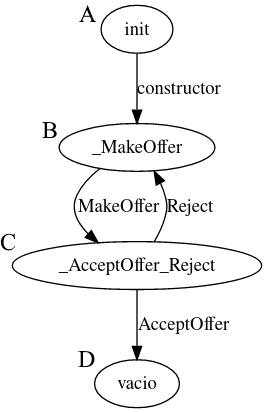
\includegraphics{figs/simple-merketplace-epa.png}
        \caption{EPA de \texttt{SimpleMarketplace}. Las etiquetas en los estados indican los métodos que se encuentran habilitados. Las etiquetas en las transiciones indican el método por el que ocurre la transición.}
        \label{fig:epa-example}
    \end{subfigure}
\end{figure}

\section{Modelo Formal}
Dado que trabajaremos sobre el código fuente de un contrato escrito en Solidity, nos interesa formalizar qué aspectos del contrato consideraremos relevantes.
Para obtener una discusión más detallada de estas formalizaciones de los artefactos de código, referirse a De Caso et. al.  \cite{de-caso-epa}.
Asimismo, la abstracción presentada del comportamiento de los contratos inteligentes origina en Godoy et. al. \cite{predicate-abstraction-for-smart-contract-validation}.
En esta sección solamente presentamos una compatibilización de los formalismos para facilitar la discusión de las EPAs más adelante.

Dicho eso, llamaremos \textit{configuraciones} a las posibles combinaciones de las variables de estado del contrato y de la blockchain, y notaremos $C$ al conjunto de todas las posibles configuraciones.

\begin{definition}(Formalización de un contrato inteligente)
    \label{definicion-smart-contract}
    Definimos a un contrato inteligente como la tupla $SC = \langle M, F, R, inv, init \rangle$ donde:

    \begin{itemize}
        \item $M = {m_1, \dots m_n}$ es el conjunto finito de métodos externos definidos en la interfaz del contrato
        \item $F$ es un conjunto de funciones indexadas por $M$. \\
              Para cada $m \in M$, $F_m : C \times \mathds{Z} \rightarrow (C \cup \bot)$ es la implementación del método $m$.
        \item $R$ es un conjunto de precondiciones indexado por $M$.\\
              Para cada $m \in M$, $R_m : C \times \mathds{Z} \rightarrow \{$\textbf{true}, \textbf{false}$\}$ indica si el método $m$ está habilitado para la configuración y parámetros indicados
        \item $inv : C \rightarrow \{$\textbf{true}, \textbf{false}$\}$ indica si una configuración cumple el invariante del contrato
        \item $init : C \rightarrow \{$\textbf{true}, \textbf{false}$\}$ indica si una configuración puede ser resultante de ejecutar el constructor del contrato
    \end{itemize}
\end{definition}

Una particularidad presente en los métodos de los contratos inteligentes es que algunas instrucciones como \textcolor{magenta}{\texttt{msg.sender}}, \textcolor{magenta}{\texttt{msg.value}}, \textcolor{magenta}{\texttt{tx.gasprice}} o \textcolor{magenta}{\texttt{tx.origin}}
\footnote{\textcolor{magenta}{\texttt{msg.value}} indica cuánto Ether está recibiendo el contrato. \textcolor{magenta}{\texttt{tx.gasprice}} indica cuánto Ether se le cobra al remitente por cada unidad de gas (cómputo) utilizada y \textcolor{magenta}{\texttt{tx.origin}} se refiere a el usuario humano que haya enviado el mensaje que disparó la ejecución actual.} hacen referencia a variables de la blockchain.
Sin embargo podemos modelar estas variables, junto con los parámetros explícitos como input codificable en $\mathds{Z}$ (los números enteros) sin pérdida de generalidad \cite{de-caso-epa}.
La semántica de un contrato la definimos como el siguiente Labeled Transition System:

\begin{definition}\label{definicion-lts}(Semántica de un contrato inteligente)
    Dado $SC = \langle M, F, R, inv, init \rangle$ un contrato inteligente, su semántica está provista por el LTS concreto $L_c = \langle \sigma , S_c, S_{0c}, \Delta _c \rangle$ que satisfaga:
    \begin{itemize}
        \item $S_c = \{conf | conf \in C \land inv(conf) = \textbf{true}\}$
        \item $S_{0c} = \{conf | conf \in S_c \land init(conf) = \textbf{true}\}$
        \item $\sigma = (F \times \mathds{Z}) \cup \tau$ es el conjunto de todos los posibles llamados a funciones, junto con un elemento $\tau$ que representa un cambio en la blockchain que ocurra de manera independiente al contrato
        \item $\Delta _c \subseteq S_c \times \sigma \times S_c$
        \item $\forall s_1,s_2 \in S_c, m \in M, z \in \mathds{Z} . \\ (s_1,(F_m,z),s_2) \in \Delta _c \iff \bigg( R_m(s_1,z) = \textbf{true} \land   F_m(s_1,z) = s_2 \bigg)$ \\
              $(s_1,\tau,s_2) \in \Delta _c \iff$ un cambio independiente en la blockchain puede llevarnos del estado $s_1$ al estado $s_2$
    \end{itemize}
\end{definition}
Notar que para cualquier contrato, el conjunto $S_c$ de estados de su LTS concreto es infinito.
Esto es porque las configuraciones tienen en cuenta variables de la blockchain externas al contrato.
Incluso para contratos donde las configuraciones de las variables internas es finita, siempre habrá infinitas configuraciones de las variables externas.
\\

A la EPA (es decir, el LTS abstracto) la definimos entonces de la siguiente manera:

\begin{definition}\label{definicion-epa}(Enabledness-Preserving-Abstraction) Dado $SC = \langle M, F, R, inv, init \rangle$ un contrato inteligente y $L_c = \langle \sigma , S_c, S_{0c}, \Delta _c \rangle$ su LTS concreto, entonces el LTS asbtracto $L_A = \langle M \cup \hat{\tau} , 2^M, P_0, \Delta _A \rangle$ es una EPA del contrato y $\alpha : S_c \rightarrow 2^M$ es la función de abstracción, donde se cumple que:
    \begin{itemize}
        \item $2^M$ es el conjunto de partes de $M$
        \item $\forall s \in S_c \: . \:
                  \alpha(s) = \{m | m \in M \land \exists z \in \mathds{Z} . R_m(s,z) = \textbf{true}\}$
        \item $P_0 = \{\alpha(s_0) | s_0 \in S_{0c} \}$
        \item $\forall s_1,s_2 \in S_c, m \in M, z \in \mathds{Z} . \\ (s_1,(F_m,z),s_2) \in \Delta _c \Rightarrow (\alpha(s_1),R_m,\alpha(s_2)) \in \Delta _A$ \\
              $(s_1,\tau,s_2) \in \Delta _c \Rightarrow (\alpha(s_1),\hat{\tau},\alpha(s_2)) \in \Delta _A$
    \end{itemize}
\end{definition}

El conjunto de estados de la \textit{EPA} es $2^M$ (el conjunto de partes de las precondiciones).
La \textit{función de abstracción} de los estados $s_c$ del LTS concreto a los estados abstractos es $\alpha (s_c) = $ ``el conjunto de métodos cuyas precondiciones son satisfechas por $s_c$''.
Una transición en la EPA entre los estados $s$ y $s'$ etiquetada con el método $m$ significa que existen algún estado concreto $s_c$ y un valor de entrada $z$ para los que $\alpha(s_c) = s$ y  $F_m(s,z)=s_c'$ con $\alpha(s_c') = s'$.
Es decir que algún llamado de $m$ a un estado que se abstrae a $s$ nos da de resultado otro estado que se abstrae a $s'$.
Una transición de $s$ a $s'$ etiquetada  con $\hat{\tau}$, la versión abstracta de $\tau$, indica que existe un estado concreto $s_c$ con $\alpha(s_c) = s$ y que puede ocurrir $\alpha (\tau (s_c)) = s'$.
